% This is "sig-alternate.tex" V2.1 April 2013
% This file should be compiled with V2.5 of "sig-alternate.cls" May 2012
%
% This example file demonstrates the use of the 'sig-alternate.cls'
% V2.5 LaTeX2e document class file. It is for those submitting
% articles to ACM Conference Proceedings WHO DO NOT WISH TO
% STRICTLY ADHERE TO THE SIGS (PUBS-BOARD-ENDORSED) STYLE.
% The 'sig-alternate.cls' file will produce a similar-looking,
% albeit, 'tighter' paper resulting in, invariably, fewer pages.
%
% ----------------------------------------------------------------------------------------------------------------
% This .tex file (and associated .cls V2.5) produces:
%       1) The Permission Statement
%       2) The Conference (location) Info information
%       3) The Copyright Line with ACM data
%       4) NO page numbers
%
% as against the acm_proc_article-sp.cls file which
% DOES NOT produce 1) thru' 3) above.
%
% Using 'sig-alternate.cls' you have control, however, from within
% the source .tex file, over both the CopyrightYear
% (defaulted to 200X) and the ACM Copyright Data
% (defaulted to X-XXXXX-XX-X/XX/XX).
% e.g.
% \CopyrightYear{2007} will cause 2007 to appear in the copyright line.
% \crdata{0-12345-67-8/90/12} will cause 0-12345-67-8/90/12 to appear in the copyright line.
%
% ---------------------------------------------------------------------------------------------------------------
% This .tex source is an example which *does* use
% the .bib file (from which the .bbl file % is produced).
% REMEMBER HOWEVER: After having produced the .bbl file,
% and prior to final submission, you *NEED* to 'insert'
% your .bbl file into your source .tex file so as to provide
% ONE 'self-contained' source file.
%
% ================= IF YOU HAVE QUESTIONS =======================
% Questions regarding the SIGS styles, SIGS policies and
% procedures, Conferences etc. should be sent to
% Adrienne Griscti (griscti@acm.org)
%
% Technical questions _only_ to
% Gerald Murray (murray@hq.acm.org)
% ===============================================================
%
% For tracking purposes - this is V2.0 - May 2012

\documentclass{sig-alternate-05-2015}


%
\def\sharedaffiliation{%
\end{tabular}
\begin{tabular}{c}}
%
\begin{document}

% Copyright
\setcopyright{acmcopyright}
%\setcopyright{acmlicensed}
%\setcopyright{rightsretained}
%\setcopyright{usgov}
%\setcopyright{usgovmixed}
%\setcopyright{cagov}
%\setcopyright{cagovmixed}


% DOI
\doi{10.475/123_4}

% ISBN
\isbn{123-4567-24-567/08/06}

%Conference
\conferenceinfo{HRI '17}{March 6--9, 2017, Vienna Austria}

\acmPrice{\$15.00}

%
% --- Author Metadata here ---
\conferenceinfo{HRI}{'2017 Vienna, Austria}
%\CopyrightYear{2007} % Allows default copyright year (20XX) to be over-ridden - IF NEED BE.
%\crdata{0-12345-67-8/90/01}  % Allows default copyright data (0-89791-88-6/97/05) to be over-ridden - IF NEED BE.
% --- End of Author Metadata ---

% \title{Towards the Understanding of Human Movement Variability with NAO as an Dance Instructor}
% \title{Towards The Classification of Human Movement Variability in Dance Activities Using NAO as an Instructor}
% \title{Towards The Classification of Movement Variability For Simple Arm Activities Using NAO as an Instructor}
% \title{Can humanoids robots teach humans how to move?}
% \title{Can a robot teach you how well you move?}
% \title{Can NAO be used to improve the quality of movement?}
% \title{Can NAO be used to analyse the quality of simple movement?}
% \title{DRAFT: Can NAO be used as a model of simple movement to analyse the variability 
% of movement?}
% \title{DRAFT: Can a humanoid-robot 
% be used as a model of simple movement to analyse the movement variability 
% accross participants and across movements?}
% \title{Can NAO be used to quantify the of simple movements across ?}
% \title{How do you know if you are copying a simple movement well?}
% \title{Can NAO be used as a instructor to
% to quantify the similarity of simple movements between humans and robot ?}
%\title{Towards the quantification of synchronisation of 
%simple movements between humans and NAO?}

% \title{Towards the Measurament of Human Motion Imitaion
% with Inertial Sensors Using a Humanoid Robot}
\title{Towards the Measurement of Human-Robot Imitation Using Wearable Inertial Sensors}



% \subtitle{[Extended Abstract]
% \titlenote{A full version of this paper is available as
% \textit{Author's Guide to Preparing ACM SIG Proceedings Using
% \LaTeX$2_\epsilon$\ and BibTeX} at
% \texttt{www.acm.org/eaddress.htm}}}
%
% You need the command \numberofauthors to handle the 'placement
% and alignment' of the authors beneath the title.
%
% For aesthetic reasons, we recommend 'three authors at a time'
% i.e. three 'name/affiliation blocks' be placed beneath the title.
%
% NOTE: You are NOT restricted in how many 'rows' of
% "name/affiliations" may appear. We just ask that you restrict
% the number of 'columns' to three.
%
% Because of the available 'opening page real-estate'
% we ask you to refrain from putting more than six authors
% (two rows with three columns) beneath the article title.
% More than six makes the first-page appear very cluttered indeed.
%
% Use the \alignauthor commands to handle the names
% and affiliations for an 'aesthetic maximum' of six authors.
% Add names, affiliations, addresses for
% the seventh etc. author(s) as the argument for the
% \additionalauthors command.
% These 'additional authors' will be output/set for you
% without further effort on your part as the last section in
% the body of your article BEFORE References or any Appendices.

\numberofauthors{2} %  in this sample file, there are a *total*
% of EIGHT authors. SIX appear on the 'first-page' (for formatting
% reasons) and the remaining two appear in the \additionalauthors section.
%
\author{
% You can go ahead and credit any number of authors here,
% e.g. one 'row of three' or two rows (consisting of one row of three
% and a second row of one, two or three).
%
% The command \alignauthor (no curly braces needed) should
% precede each author name, affiliation/snail-mail address and
% e-mail address. Additionally, tag each line of
% affiliation/address with \affaddr, and tag the
% e-mail address with \email.
%
\alignauthor XXX%Miguel P. Xochicale\\
      \email{xxx@bham.ac.uk}%\email{map479@bham.ac.uk}
%
\alignauthor XXX\\ %Chris Baber\\
      \email{xxx@bham.ac.uk}%\email{c.baber@bham.ac.uk}
%
      \sharedaffiliation
      \affaddr{School of XXX}  \\%\affaddr{School of Electronic, Electrical and Systems Engineering}  \\
      \affaddr{University of Birmingham}   \\
      \affaddr{Birmingham, B15 2TT, UK}
% 1st. author
%
%
% % % \alignauthor
% % % Miguel P. Xochicale \\
% % % \affaddr{University of Birmingham}\\
% % % \affaddr{Birmingham, B15 2TT, UK}\\
% % % \email{perez.xochicale@gmail.com}
% % % % 2nd. author
% % % \alignauthor
% % % Chris Baber\titlenote{Electronic, Electrical and Systems Engineering, University of Birmingham, Birmingham, UK}\\
% % % \affaddr{University of Birmingham}\\
% % % \affaddr{Birmingham, B15 2TT, UK}\\
% % % \email{c.baber@bham.ac.uk}
%
%       
% % 3rd. author
% \alignauthor 
% XXX XXX\titlenote{xxxx xxxxx xxxx xxxxx xxxx xxxxx xxxx xxxxx}\\
%        \affaddr{University of XXX}\\
%        \affaddr{XXX,XXX}\\
%        \email{xxx@xxx.xxx}
}
% There's nothing stopping you putting the seventh, eighth, etc.
% author on the opening page (as the 'third row') but we ask,
% for aesthetic reasons that you place these 'additional authors'
% in the \additional authors block, viz.
% \additionalauthors{Additional authors: John Smith (The Th{\o}rv{\"a}ld Group,
% email: {\texttt{jsmith@affiliation.org}}) and Julius P.~Kumquat
% (The Kumquat Consortium, email: {\texttt{jpkumquat@consortium.net}}).}
% \date{30 July 1999}
% Just remember to make sure that the TOTAL number of authors
% is the number that will appear on the first page PLUS the
% number that will appear in the \additionalauthors section.

\maketitle
\begin{abstract}
% How close you imitate a robot can be used as a metric of quality of movement.
In this study, we use inertial sensors attached both to a humanoid-robot
and to a person in order to quantify how close a participant imitates 
a robot. Twelve healthy participants were invited to perform 
simple arm movements for which we applied a propose framework based
on non-linear dynamics to capture the non-linear structure of the time-series
and PCA to reconstruct the state space.
It turns out that participants show different ranges of the proposed metric
which can be linked with to level of imitation.
Such proposal can be useful in determining a detailed scoring of human-robot imitation
during training or rehabilitation.



% Due to different amplitudes and periods when repiting 
% non-linear properties of the structure of time-series
% that 

% a sample of a \LaTeX\ document which conforms,
% somewhat loosely, to the formatting guidelines for
% ACM SIG Proceedings. It is an {\em alternate} style which produces
% a {\em tighter-looking} paper and was designed in response to
% concerns expressed, by authors, over page-budgets.
% It complements the document \textit{Author's (Alternate) Guide to
% Preparing ACM SIG Proceedings Using \LaTeX$2_\epsilon$\ and Bib\TeX}.
% This source file has been written with the intention of being
% compiled under \LaTeX$2_\epsilon$\ and BibTeX.
\end{abstract}


%
% The code below should be generated by the tool at
% http://dl.acm.org/ccs.cfm
% Please copy and paste the code instead of the example below. 
%
\begin{CCSXML}
<ccs2012>
<concept>
<concept_id>10010520.10010553.10010554.10010558</concept_id>
<concept_desc>Computer systems organization~External interfaces for robotics</concept_desc>
<concept_significance>500</concept_significance>
</concept>
</ccs2012>
\end{CCSXML}

\ccsdesc[500]{Computer systems organization~External interfaces for robotics}


%
% End generated code
%

%
%  Use this command to print the description
%
\printccsdesc

% We no longer use \terms command
%\terms{Theory}

% \keywords{ACM proceedings; \LaTeX; text tagging}
\keywords{Human-Robot Imitation, Movement Variability, Wearable sensors, Inertial sensors,
Non-linear Dynamics}

\section{Introduction}
Recently, NAO, a humanoid robot, has successfully been used either as a fitness coach for elderly 
or as an instructor of rehabilitation for children.
For instance, the work of G{\"{o}}rer \textit{et al.} takes advantage of an RGB-D camera to 
extract joint angles of a human demonstrator and participants in order to
compute the absolute differences between them \cite{Gorer2016}. Such absolute differences
in joint angles are useful to create a corrective feedback for the movement of the elderly 
with regard to (i) speed adjustment, (ii) amplitude adjustment, (iii) mirroring detection
and (iv) no motion.
However, on one hand, when participants are seated the RGB-D camera cannot provide correct skeleton information,
and, on the other hand, there is room for implementation of a detailed scoring of human-robot imitation.
Guneysu \textit{et al.} used NAO and wearable inertial sensors
to monitor arm rehabilitation motions in children \cite{Guneysu2015}.
The challenge for Guneysu \textit{et al.} is to keep the children's motivation in order to imitate 
movements for arm rehabilitation therapy. For this, in their previous study they used Kinect sensor
to compute joint angles of motion but when therapists interact with children they obstruct 
the kinect sensor to which inertial sensors were used in order 
to avoid obstructions between the children, the therapist and  the robot.
However, as part of their study, it turns out that four physiotherapists have their own way to move
when they were asked to perform the arm motions
which is reflected in the differences of frequency and amplitude of the movements
as well as the initial positions of the hands.

For this study, we are therefore proposing 
the use of inertial sensors to avoid any obstructions when using video-based sensors
and the use of NAO to control simple movements that participants are going to imitate.
Similarly, we are proposing a framework based on a non-linear dynamic technique and PCA
in order to explore 
% how to  analyse the data collected from inertial
% sensors attached both to a humanoid-robot and to a person
% in order to quantify 
how close the participants mimic the original movement of the robot.


% measure human-robot imitation 
% and to explore the similarity of movements across participants.


% which can be used as a metric on how close the participant mimics the original movement 
% of the robot.



% For our exploration purposes of movement variability, we adopt the Sequence-Base Model
% in which the movement sequences are created by the teacher and the pupils
% reproduce it in the same way.
% It is important to note that the teaching methodology is the same but the movements performed
% by users were completely different between sessions.
% However, there is no analysis about the quantification of the quality of the
% improvement of the movements as children performed in each of the three sessions 
% but only a score for accommodation that is a ratio between the number of times when robot shows and asks
% for a motion of the user \cite{Ros2014}.





% 
% 
% 
% Chen et al. proposed a tennis swing training using accelerometer sensors which classifies 
% four categories of motion 
% (correct forehand swings, only swing wrist, arm unstretchable and racket is not vertical) 
% with a ID3 inductive learning algorithm \cite{Chen2010}.







\section{METHODS}

\subsection{Research Questions}

How to use and analyse the data collected from inertial sensors attached both 
to a humanoid-robot and to a person in order to quantify how close a participant 
imitates a robot?
% with different participants performing different simple movements?
% How the variability of a movement can be related to the dexterity of the performance
% of such movement?


\subsection{Hypotheses}
With this preliminary study, we expect to generate an intuitive 
explanation of the problem of measurement of human-robot imitation 
in order to provide metrics on how close a participant can imitate the original
movement.
% In the same vein
% which 
% at the same time can help us to establish the base line of movements
% to quantify the variability accross partipants and between movements.
%   can be linked with the leve dexterity of users and more 
%   importantly provide feedback to move better.


% the human-robot motion imitation. 

\subsection{Participants}
Twelve healthy participants (two females and ten males)
mean age 19.5$\pm$0.79 (from now on abbreviated as p01 to p12) were invited to 
participate in this study. All the participants were right handed.
The design of the experiment was approved by University of Birmingham ethics approval
process. All participants provided informed consent forms prior to participation.



\subsection{Procedure}
Participants were asked to imitate two simple arm movements: (i) 
horizontal movement (Figure~\ref{fig:main}-A) and (ii) vertical movement;
such simple movements were performed by NAO and each movement were repeated ten times
for both the robot and the participant.
Data were then collected at a sampling rate of 50Hz with two NeMEMSi inertial sensors
which provide tri-axial data of accelerometer, gyroscope and magnetometer sensors and
quaternions \cite{Comotti2014}. Because of the front to front imitation activity, 
inertial sensors were attached the right hand of the participant and to the left hand of the robot.

It is important to note that due to the reduced space, we are only presented
results for the horizontal movement and 
we focus our analysis on the $z$ axis from the gyroscope sensor ($g_z$) 
which is mostly affected by the nature of the horizontal movement (Figure~\ref{fig:main}-A).

% Due to the simplicity of the proposed movements  in this study, 
% (Figure~\ref{fig:main}-A).








\section{State Space reconstruction}
The proposed framework to measure human-robot imitation
is based on the method of time-delay embedding and PCA.
% which mainly increase the dimensionally of the data, 
% $\mathbb{R} \rightarrow \mathbb{R}^m$,
% then a further transformation is considered,
% $\mathbb{R}^m \rightarrow \mathbb{R}^n$, 
% which for our study is PCA due to its non-parametric feature.
Our motivation to use the method of time-delay embedding
is due to the non-linear structure of the time-series.
Such non-linear structure is presented in different periods and amplitudes 
between repetitions of movements and across movements of participants (Figure~\ref{fig:main}-B,C).
Similarly, we use PCA as a method for dimensionality reduction due to its non-parametric feature.
% , we use the time-delay embedding
% as our main method for this study in order to measure the human-robot motion imitation.
The method of time-delay embedding is an array of 
time delayed copies of the available time series $x(n)$ and is defined as  
$ \overline{x}(n) = \{  x(n), x(n-\tau), x(n-2\tau), \dots,x(n-(m-1)\tau)\}$
where $m$ is the embedding dimension and $\tau$ is the delay embedding \cite{Huke2006}.
We then applied PCA to $ \overline{x}(n)$ in order to get $PC_1, PC_2, \dots, PC_m$ 
to which we use $PC_1$ and $PC_2$ 
to create a state space reconstruction (Figure~\ref{fig:main}-D,E and F).
Finally, we computed euclidean distances in the state space 
from (0,0) point to each ($PC_1(i),PC_2(i)$) point where $1 \leq i \leq m$
in order to obtain the box-and-whisker plots for each participant (Figure~\ref{fig:main}-G).




\section{PRELIMINARY RESULTS}



We want to emphasise that the use of the time-delay embedding 
method in order to characterise the non-linearities of the time-series 
and the use of PCA as a tool for dimensionality 
reduction is useful to measure how close participants 
imitate the original movement from the robot.


On one hand, it is expect that the robot performs very similar repetitions of movements 
which are visualised in the orange time-series
Therefore, a tight circular  shape of the reconstructed state space (Figure~\ref{fig:main}-D)
is linked with little interquartile range of the respective box-and-whisker plot  (Figure~\ref{fig:main}-G).
On the other hand, 
the time-series of participant 05 shows (Figure~\ref{fig:main}-C)
 different amplitude and periods per repetitions which
are related to the disjointed circular shape of 
the reconstructed state space (Figure~\ref{fig:main}-F) and therefore 
linked with a maximum interquartile range in the  box-and-whisker plots  (Figure~\ref{fig:main}-G).

We also show that participant 01 is an example of a good imitator of the robot movement
(Figure~\ref{fig:main}-B,E and G).




\begin{figure}[ht]
\centering
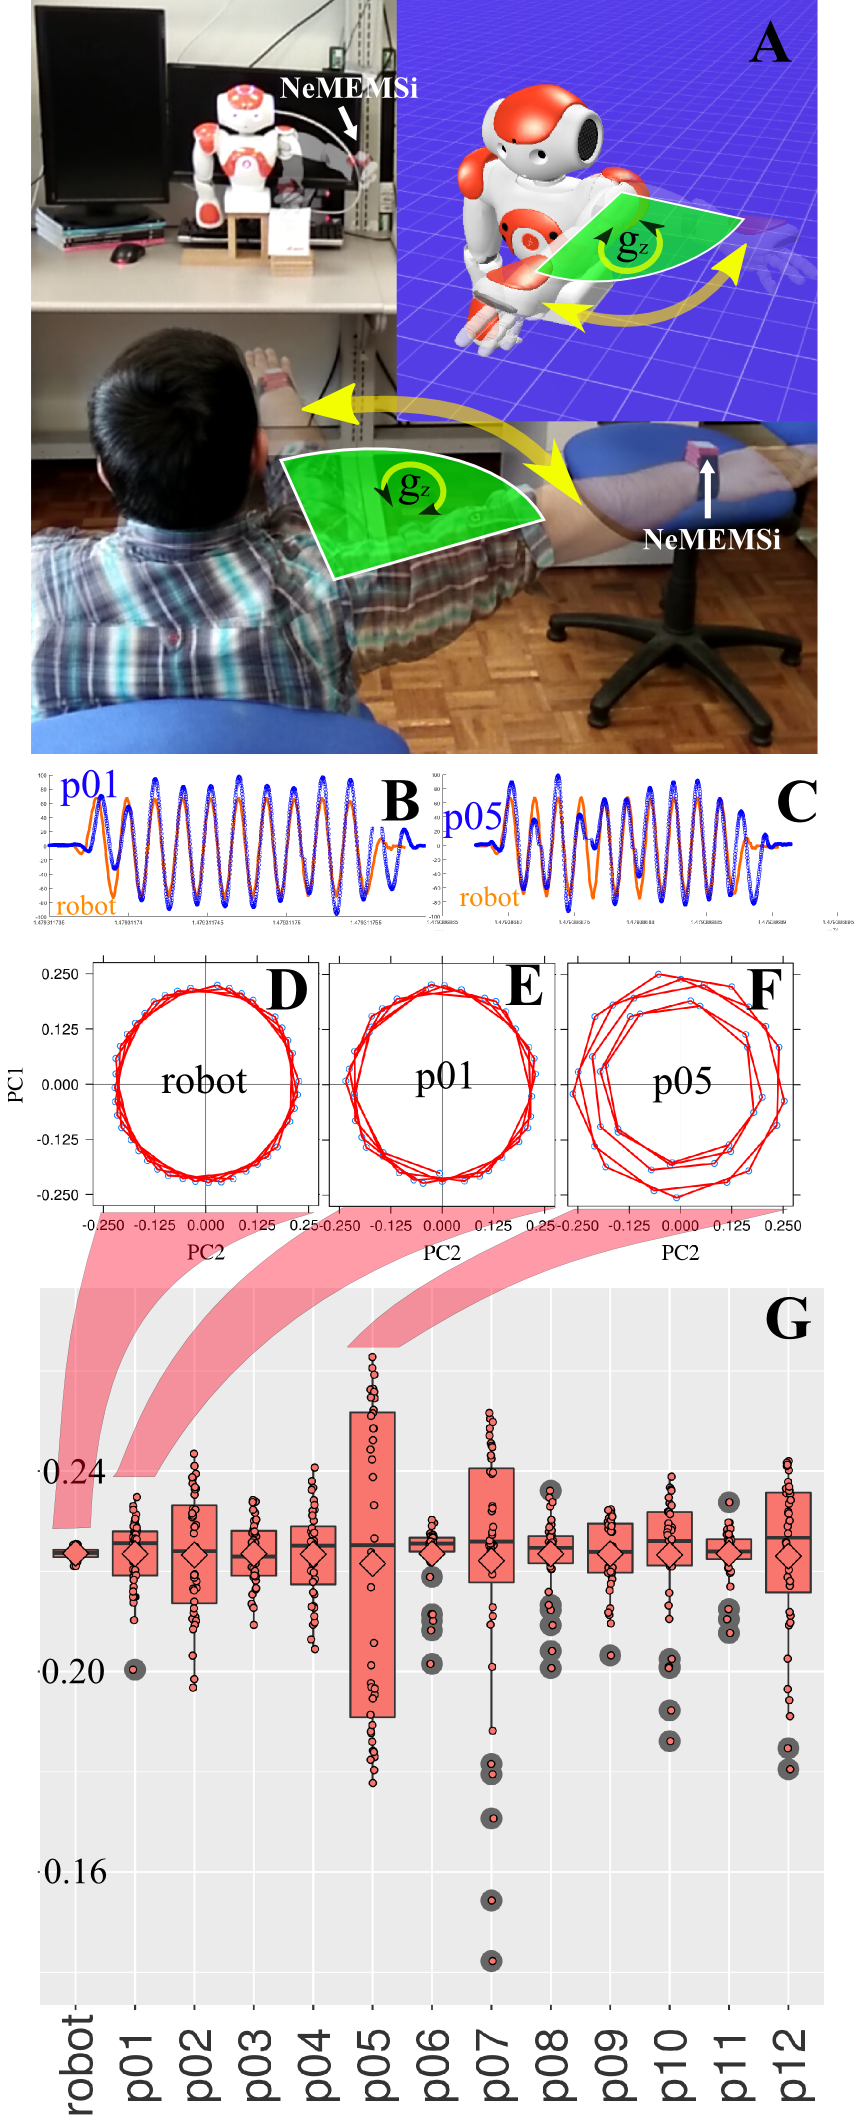
\includegraphics[width=0.27\textwidth]{fig06}
\caption{
NAO and participant performing the horizontal movement (A). 
Smoothed angular acceleration $g_z$ for participant 01  and robot (B)
and for participant 05 and robot (C).
Reconstructed state spaces  ($m=40$, $\tau=10$) for robot (D), participant 01 (E) and participant 05 (F).
Euclidean distances from the reconstructed state space for the robot and twelve participants (G).
}
\label{fig:main}
\end{figure}






\section{FUTURE WORK}
One our main concerns when quantifying human-robot imitation
is the lack of metrics to say who can be considered a bad, intermediate or good imitator.

For future work, there are four areas that we are going to investigate:
(i) data collection from a wider range of individuals (gender and age)
and from additional inertial sensors attached to the body,
(ii) explore complex movements which can be performed by both NAO and persons,
(iii) undertake a wider review of non-linear techniques that can be used for 
the assessment of human-robot imitation, and, 
(iv) explore the use of convolutional neural networks for automatic 
classification of the levels of human-robot imitation.


% participants whom will perform complex movements in groups.
% Take advantage of the Deep Neural Networks to automatically clasify the quality of the movements 
% according to how well the participants are in sync with the movements.
%\end{document}  % This is where a 'short' article might terminate

% %ACKNOWLEDGMENTS are optional
% \section{Acknowledgments}
% XX XX is supported by XXX. The support
% is gratefully acknowledged
% %


% The following two commands are all you need in the
% initial runs of your .tex file to
% produce the bibliography for the citations in your paper.
\bibliographystyle{abbrv}
\bibliography{literature}  % sigproc.bib is the name of the Bibliography in this case
% You must have a proper ".bib" file
%  and remember to run:
% latex bibtex latex latex
% to resolve all references
%
% ACM needs 'a single self-contained file'!
%


% %APPENDICES are optional
% %\balancecolumns
% \appendix
% %Appendix A
% \section{Headings in Appendices}
% The rules about hierarchical headings discussed above for
% the body of the article are different in the appendices.
% In the \textbf{appendix} environment, the command
% \textbf{section} is used to
% indicate the start of each Appendix, with alphabetic order
% designation (i.e. the first is A, the second B, etc.) and
% a title (if you include one).  So, if you need
% hierarchical structure
% \textit{within} an Appendix, start with \textbf{subsection} as the
% highest level. Here is an outline of the body of this
% document in Appendix-appropriate form:
% \subsection{Introduction}
% \subsection{The Body of the Paper}
% \subsubsection{Type Changes and  Special Characters}
% \subsubsection{Math Equations}
% \paragraph{Inline (In-text) Equations}
% \paragraph{Display Equations}
% \subsubsection{Citations}
% \subsubsection{Tables}
% \subsubsection{Figures}
% \subsubsection{Theorem-like Constructs}
% \subsubsection*{A Caveat for the \TeX\ Expert}
% \subsection{Conclusions}
% \subsection{Acknowledgments}
% \subsection{Additional Authors}
% This section is inserted by \LaTeX; you do not insert it.
% You just add the names and information in the
% \texttt{{\char'134}additionalauthors} command at the start
% of the document.
% \subsection{References}
% Generated by bibtex from your ~.bib file.  Run latex,
% then bibtex, then latex twice (to resolve references)
% to create the ~.bbl file.  Insert that ~.bbl file into
% the .tex source file and comment out
% the command \texttt{{\char'134}thebibliography}.
% % This next section command marks the start of
% % Appendix B, and does not continue the present hierarchy
% \section{More Help for the Hardy}
% The sig-alternate.cls file itself is chock-full of succinct
% and helpful comments.  If you consider yourself a moderately
% experienced to expert user of \LaTeX, you may find reading
% it useful but please remember not to change it.
% %\balancecolumns % GM June 2007
% % That's all folks!



\end{document}
